\section{数据预处理与探索性分析}\label{sec:data}

\subsection{数据组织与验证划分}
原训练集包含5642条带标签记录，A、B特征表各包含1000条记录。A答案按有表头读取，B答案按无表头读取，并按文件原有行顺序与特征表匹配。三类特征表的ID互不重复；由于标签文件未含ID，该核对不能独立证明文件提供时的标签排序来源。

当前主协议将原训练集与带标签A集合并为6642条，以随机种子23按70/30划分，得到4649条训练记录和1993条开发记录。开发记录由原训练集1685条与A集308条组成，并非独立的纯A集。表\ref{tab:protocol}区分训练选型、开发评分和B评分的样本范围。
该协议利用研究阶段已取得的A集标签，用于现有数据上的扩展训练与复核，不等同于初赛仅提供原始训练标签时的在线提交协议。仅使用原训练集拟合的历史H2结果在附录\ref{app:history}中单列。
\begin{table}[htbp]
\small
\setlength{\tabcolsep}{5pt}
\centering
\caption{当前主协议的样本与拟合范围}
\label{tab:protocol}
\begin{tabular}{L{0.13\linewidth}L{0.13\linewidth}L{0.12\linewidth}L{0.5\linewidth}}
\toprule
用途 & 拟合/选择行 & 评价行 & 备注 \\
\midrule
训练内部选择 & 4649 & 相应训练验证折 & 原train3957+A692；五折内估计预处理 \\
开发评分 & 4649 & 1993 & 原train1685+A308；不是纯A验证 \\
B集复核 & 6642 & 1000 & 冻结后以train+A全部重拟合；B有历史使用 \\
\bottomrule
\end{tabular}
\end{table}


表示、参数和权重确定后，B评价使用全部6642条重新拟合模型与预处理器，再预测同一1000条B记录。开发和B评价的拟合样本数及目标分布不同，不能由B的绝对MSE较小推断模型性能随之增强。

原训练集日期为2017年9月15日至10月31日，A集为10月10日至10月31日，B集为10月20日至10月31日，日期范围相互重叠。因此，B集不等于严格未来批次。开发集及B集均有历史使用，本文将冻结后评分称为已知集合复核。

\subsection{编码、填补与表示变换}
删除预测输入中的ID与体检日期，性别固定编码为女0、男1，其余取缺失，并增加性别未知指示。39个原始预测字段在增加未知指示后形成40列基础输入；去除乙肝五项后为35列。这些维数均不包含后续自动增加的缺失指示或工程特征。

对某次拟合行集合$F$，令$m_{ij}$表示第$i$行第$j$列是否缺失，$q_j(F)$为该列在$F$中的非缺失中位数。采用填补时，定义
\begin{equation}
\widetilde x_{ij}=\begin{cases}
x_{ij},&m_{ij}=0,\\
q_j(F),&m_{ij}=1,
\end{cases}
\qquad u_i=\bigl(\widetilde x_i,(m_{ij})_{j\in J_F}\bigr),
\label{eq:impute}
\end{equation}
其中$J_F$为拟合行中出现过缺失的列集合。对拟合部分全空的列，按实现保留该列并填为0。显式性别未知指示与填补器的性别缺失指示可能重复，本文保留原实现。所有拟合统计量均来自$F$，评价记录仅应用既定变换。这与将预处理纳入训练管线的原则一致\cite{pitfalls}。

标准化在填补后的向量$u_i$上进行。对第$j$列，令$\mu_j(F)$为拟合均值，$s_j(F)$为以$n_F=|F|$作分母计算的标准差；对于零方差列或实现按浮点误差界判定为近常量的列，$s_j^*(F)$取1，其余取$s_j(F)$，则
\begin{equation}
z_{ij}=\frac{u_{ij}-\mu_j(F)}{s_j^*(F)}.
\label{eq:scale}
\end{equation}
标准化不施于血糖目标；年龄在任何缩放后仍保持浮点数，不转整数。

PCA对实际送入的训练矩阵$A_F$中心化，以其协方差矩阵的特征向量构造投影。设特征值为$\nu_1\ge\cdots\ge\nu_p$，前$r$个方向为$V_r$，则
\begin{equation}
t_i=(A_i-\overline A_F)V_r,\qquad
r=\min\left\{k:\frac{\sum_{j=1}^{k}\nu_j}{\sum_{j=1}^{p}\nu_j}>0.98\right\}.
\label{eq:pca}
\end{equation}
原基准的PCA候选先填补和标准化；第\ref{sec:preprocessing}节另比较不作单位方差缩放的PCA。PCA采用完整奇异值分解，维数由各拟合部分确定\cite{pca}，不把训练探索中的固定成分数施于所有折。

\subsection{分布、缺失与极端值}
4649条训练记录的年龄范围为3至93，均值45.718004。血糖均值5.626855，样本标准差1.474255，范围3.07至38.43；开发集与B集均值分别为5.700527和5.486880。图\ref{fig:age}及图\ref{fig:glucose}展示训练分布。血糖图中的拟合正态曲线仅作参照，较长的右尾并不支持将其视为已通过正态性检验。
\begin{figure}[htbp]
\centering
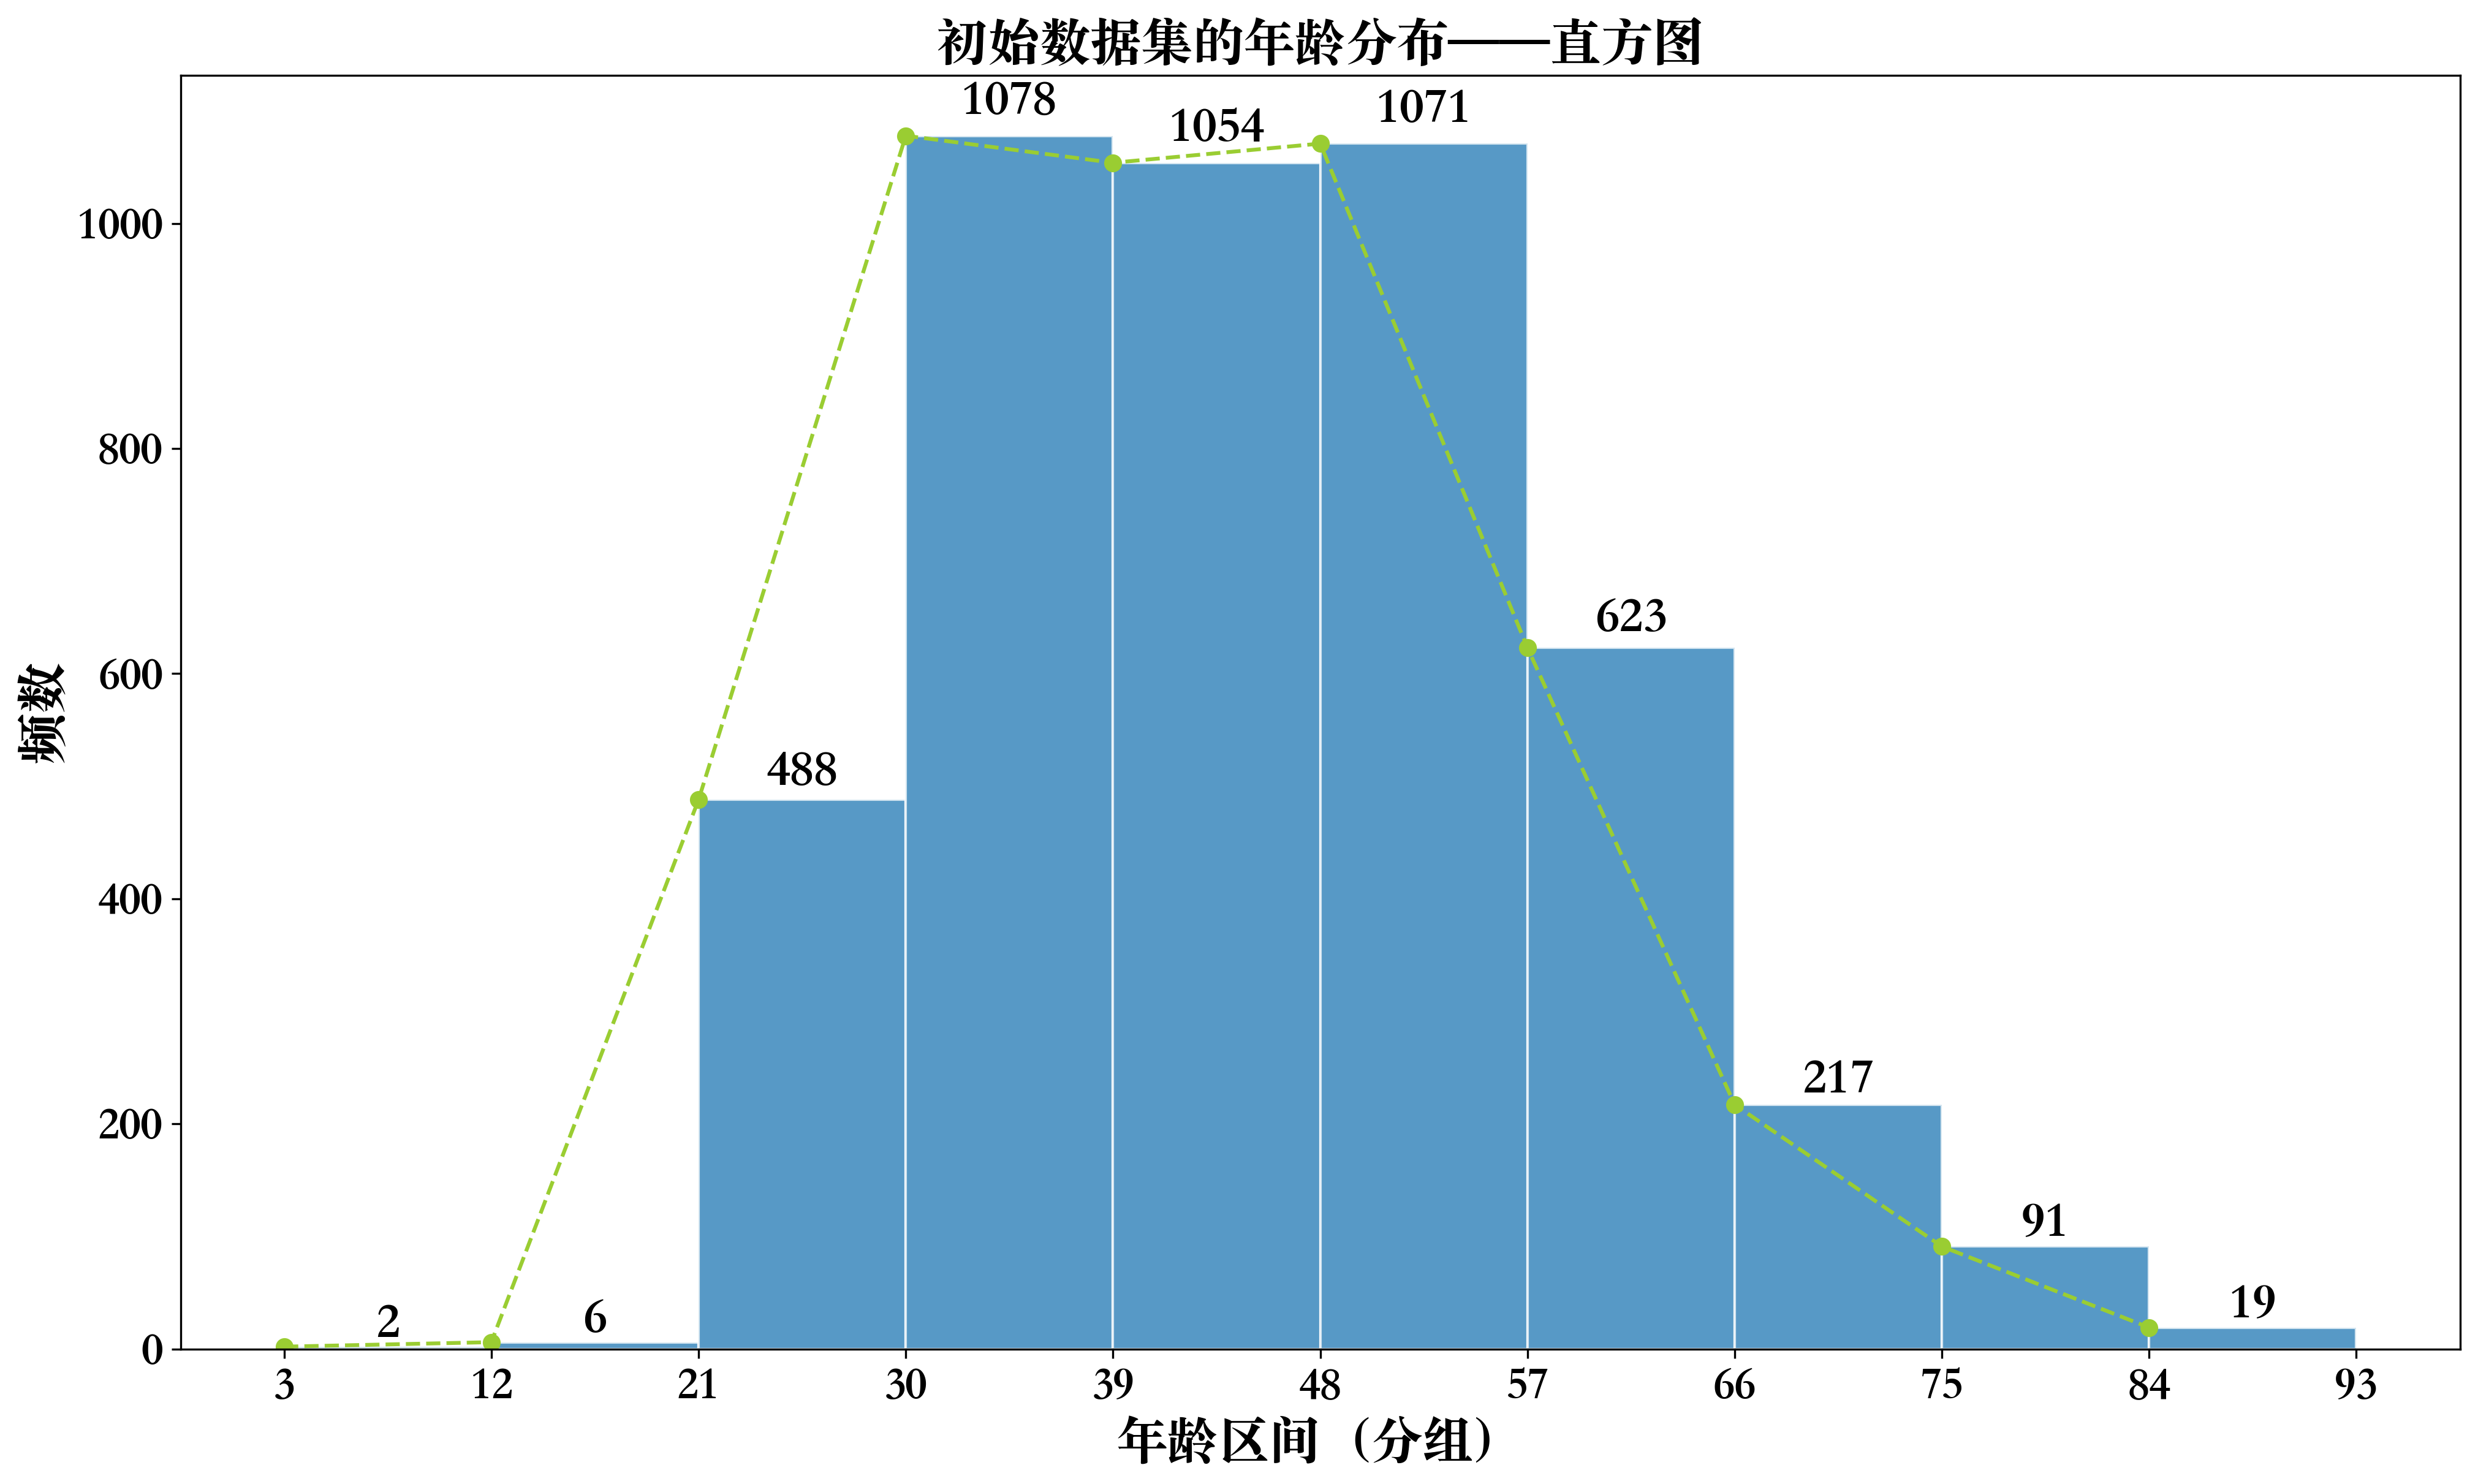
\includegraphics[width=0.94\linewidth,height=0.68\textheight,keepaspectratio]{paper/figures/paper_C007_O03.png}
\caption{4649条训练记录的年龄分布；原图标题中的初始数据指当前训练子集。}
\label{fig:age}
\end{figure}
\begin{figure}[htbp]
\centering
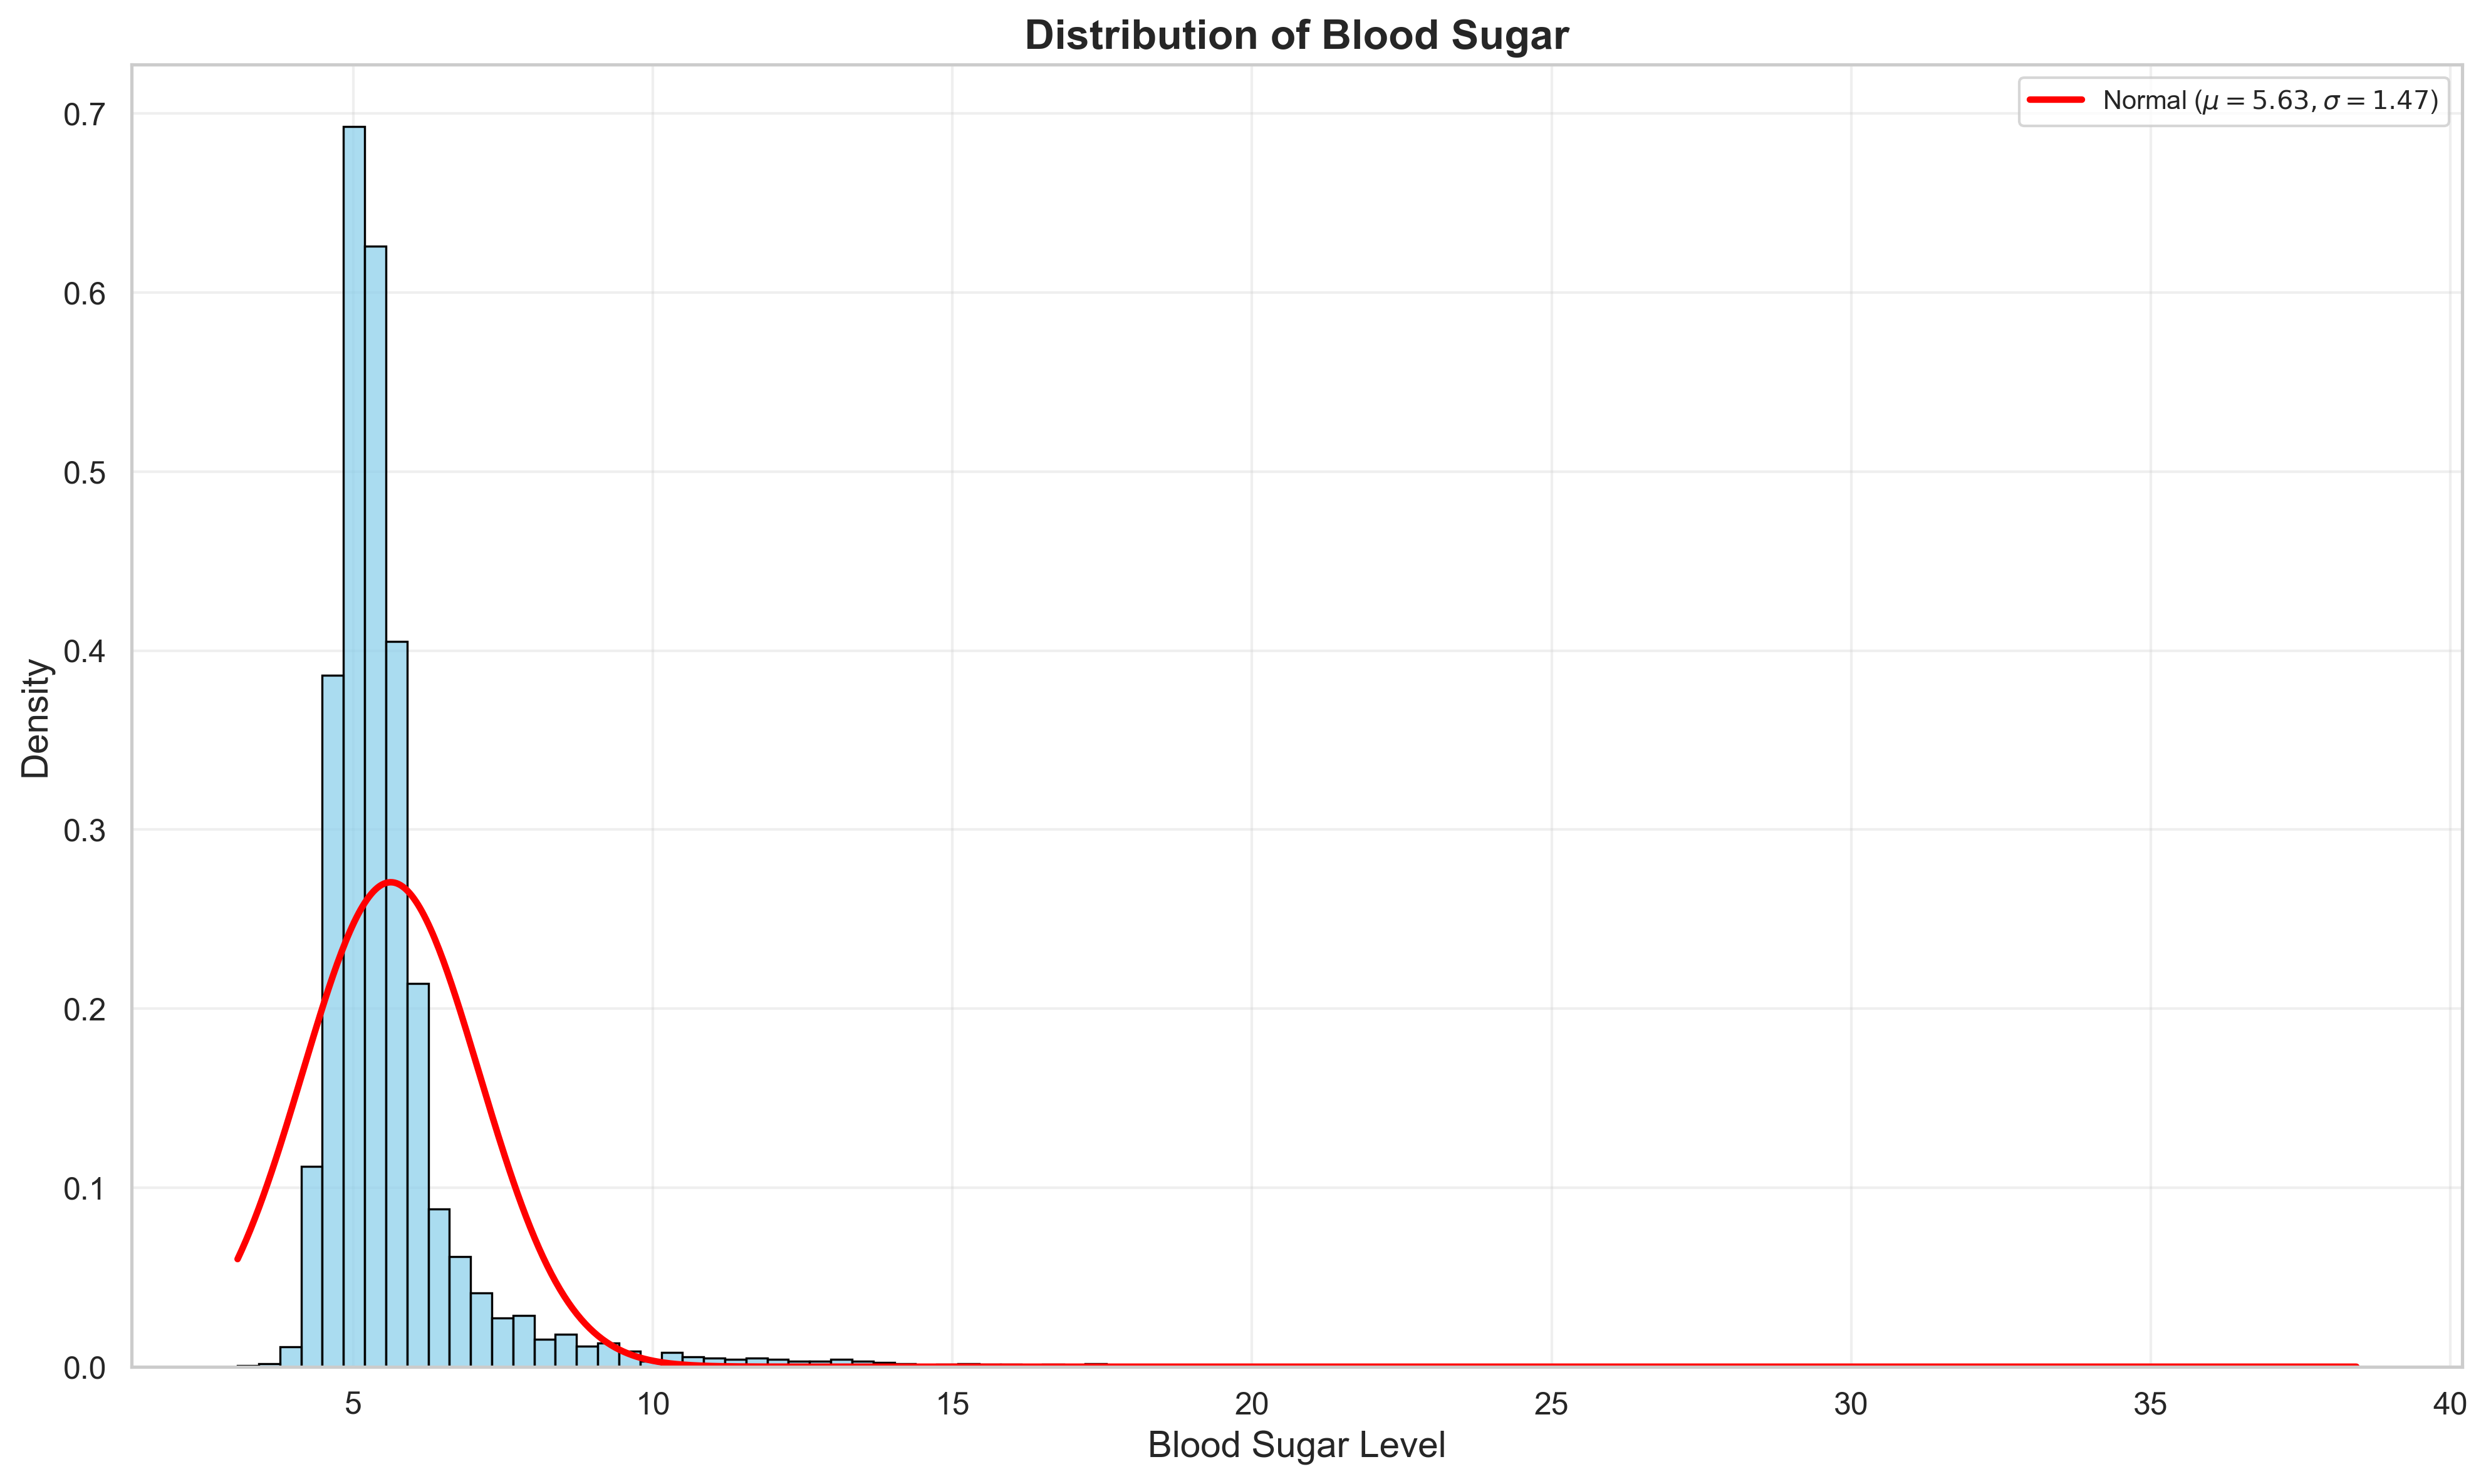
\includegraphics[width=0.94\linewidth,height=0.68\textheight,keepaspectratio]{paper/figures/paper_C009_O01.png}
\caption{4649条训练记录的血糖分布及拟合正态参照曲线；曲线不代表正态性检验结论。}
\label{fig:glucose}
\end{figure}

图\ref{fig:missing}中乙肝五项各缺失76.7047\%，尿素、肌酐、尿酸各缺失23.1233\%，部分肝功能与蛋白指标各缺失20.9507\%。按当前特征口径，1037条训练记录的缺失比例超过20\%，均保留。多个项目的共同缺失及中位数填补会影响探索相关结构，相关热图不能完全解释为生物学联系。
\begin{figure}[htbp]
\centering
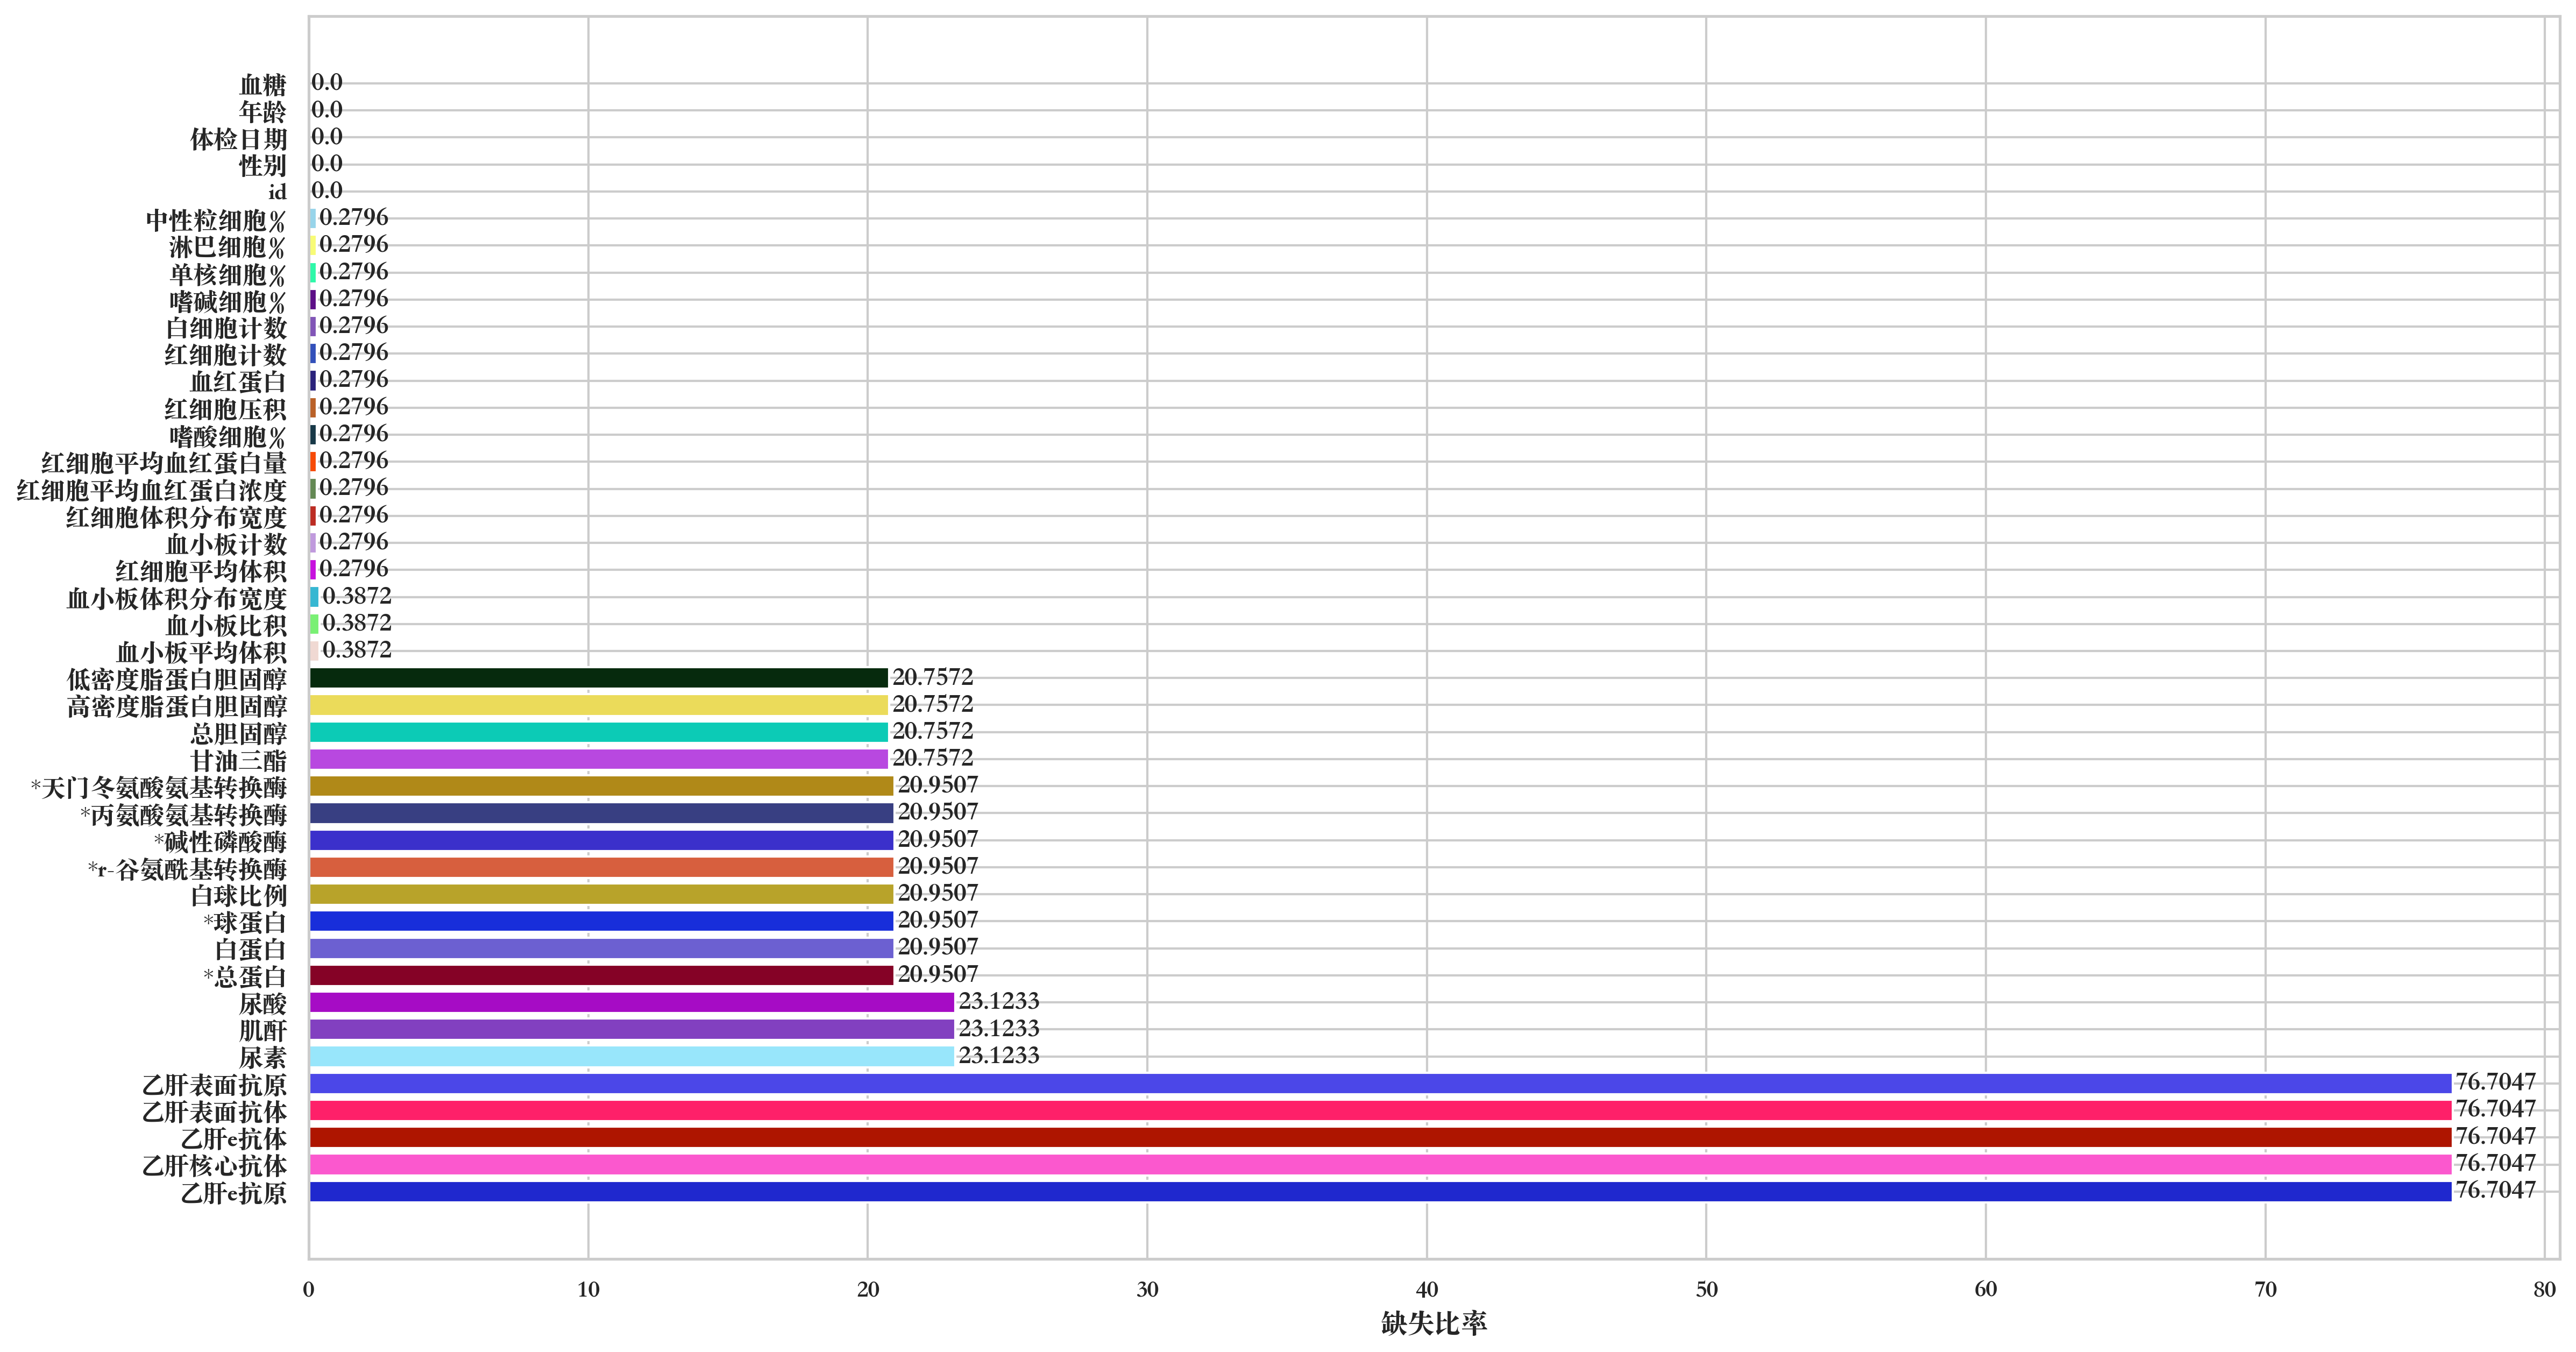
\includegraphics[width=0.94\linewidth,height=0.68\textheight,keepaspectratio]{paper/figures/paper_C012_O02.png}
\caption{4649条训练记录各列缺失比例；原样提取自缺失处理前探索。}
\label{fig:missing}
\end{figure}

探索阶段对既有检验阈值只计数，不删除样本。AST超过200有1条、ALT超过250有2条、GGT超过600有3条、血小板超过600有2条、球蛋白超过60有1条、甘油三酯超过30有2条、肌酐超过175有1条。未发现足以将这些值统一判定为录入错误的依据，故不裁剪输入或血糖目标。

\subsection{线性与降维探索}
令$\xi_i$表示训练探索副本中经中位数填补的40维基础输入，$\zeta_i$为该探索矩阵按训练均值与方差标准化后的向量。采用含截距的普通最小二乘进行拟合诊断：
\begin{equation}
(\widehat b,\widehat\beta)=\operatorname*{arg\,min}_{b,\beta}
\sum_{i\in\mathcal D_T}(y_i-b-\xi_i^\top\beta)^2.
\label{eq:ols}
\end{equation}
此处使用40列填补后的基础输入，不增加预测管线的自动缺失指示。训练MSE约1.807，$R^2$约0.168，条件数约$1.49\times10^6$；残差偏度5.884、峰度87.895。残差与Q--Q图见附录\ref{app:diagnostics}，说明线性拟合仍存在较大尾部偏差；这些训练指标不用于外部预测排名。

另在标准化训练探索输入上拟合Lasso：
\begin{equation}
(\widehat b_L,\widehat\beta_L)=\operatorname*{arg\,min}_{b_L,\beta_L}
\frac{1}{2n_T}\sum_{i\in\mathcal D_T}(y_i-b_L-\zeta_i^\top\beta_L)^2
+\alpha_L\|\beta_L\|_1,\qquad\alpha_L=0.05.
\label{eq:lasso}
\end{equation}
Lasso采用坐标下降求解，目标口径遵循实现\cite{lasso}。按系数绝对值排序，年龄、甘油三酯、红细胞平均血红蛋白浓度分别为0.296907、0.173759和0.105182。该排序是给定惩罚和表示下的稀疏线性关联，不等于最终融合的重要性，也不直接用于统一删除零系数变量。

探索PCA矩阵达到98\%累计方差约需29个成分，但其输入未包含自动缺失指示，不能将29视为所有预测管线的维数。KMO为0.469000，Bartlett计算伴随近奇异协方差和广义逆警告，相关结果仅保留为探索记录，不作为采用PCA的预测依据。

\subsection{辅助指标与结果精度}
在式\eqref{eq:mse}之外，以均方根误差、平均绝对误差和决定系数辅助分析。令$\bar y_E$为评价目标均值，则
\begin{equation}
\begin{aligned}
\operatorname{RMSE}_E&=\sqrt{\operatorname{MSE}_E},\\
\operatorname{MAE}_E&=\frac1{n_E}\sum_{i\in E}|y_i-\hat y_i|,\\
R_E^2&=1-\frac{\sum_{i\in E}(y_i-\hat y_i)^2}{\sum_{i\in E}(y_i-\bar y_E)^2}.
\end{aligned}
\label{eq:auxiliary}
\end{equation}
MSE与RMSE对应原始目标尺度的平方及一次量纲，$R^2$无量纲；原材料未提供的物理单位不另行指定。各表通常显示六位小数，以便核对存档，显示精度不代表测量精度。
